%---- IMPORTANTE ----
% Esta plantilla está basada en las recomendaciones de la guía "Trabajo fin de Grado: Escribir el TFG", que encontrarás en http://uc3m.libguides.com/TFG/escribir
% contiene recomendaciones de la Biblioteca basadas principalmente en estilos APA e IEEE, pero debes seguir siempre las orientaciones de tu Tutor de TFG y la normativa de TFG para tu titulación.
% Encontrarás un ejemplo de TFG realizado con esta misma plantilla en el archivo "ejemplo_TFG_2017.zip", incluido en la misma carpeta. Consúltalo porque contiene ejemplos útiles para incorporar tablas, figuras, listados de código, bibliografía, etc.


%----------
%	CONFIGURACIÓN DEL DOCUMENTO
%----------

\documentclass[12pt]{report} %fuente a 12pt

% MÁRGENES: 2,5 cm sup. e inf.; 3 cm izdo. y dcho.
\usepackage[
a4paper,
vmargin=2.5cm,
hmargin=3cm
]{geometry}

% INTERLINEADO: Estrecho (6 ptos./interlineado 1,15) o Moderado (6 ptos./interlineado 1,5)
\renewcommand{\baselinestretch}{1.15}
\parskip=6pt

% soporte para generar PDF/A --es importante de cara a su inclusión en e-Archivo porque es el formato óptimo de preservación y a la generación de metadatos, tal y como se describe en http://uc3m.libguides.com/ld.php?content_id=31389625. En la carpeta incluímos el archivo plantilla_tfg_2017.xmpdata en el que puedes incluir los metadatos que se incorporarán al archivo PDF cuando lo compiles. Ese archivo debe llamarse igual que tu archivo .tex
\usepackage[a-1b]{pdfx}

\usepackage{hyperref}
\hypersetup{linktoc=all}

% Expresiones matemáticas
\usepackage{amsmath,amssymb,amsfonts,amsthm}

\usepackage{txfonts} 
\usepackage[T1]{fontenc}
\usepackage[utf8]{inputenc}

\usepackage[spanish, es-tabla]{babel} % información sobre el paquete babel para español http://osl.ugr.es/CTAN/language/spanish/babel/base/spanish.pdf
\usepackage[babel, spanish=spanish]{csquotes}
\AtBeginEnvironment{quote}{\small}

% DEFINICIÓN DE COLORES para portada y listados de código
\usepackage{color}
\definecolor{azulUC3M}{RGB}{0,0,102}
\definecolor{gray97}{gray}{.97}
\definecolor{gray75}{gray}{.75}
\definecolor{gray45}{gray}{.45}

% diseño de PIE DE PÁGINA
\usepackage{fancyhdr}
\pagestyle{fancy}
\fancyhf{}
\renewcommand{\headrulewidth}{0pt}
\rfoot{\thepage}
\fancypagestyle{plain}{\pagestyle{fancy}}

% DISEÑO DE LOS TÍTULOS de las partes del trabajo (capítulos y epígrafes o subcapítulos)
\usepackage{titlesec}
\usepackage{titletoc}
\titleformat{\chapter}[block]
	{\large\bfseries\filcenter}
	{\thechapter.}
	{5pt}
	{\MakeUppercase}
	{}
\titlespacing{\chapter}{0pt}{0pt}{*3}
\titlecontents{chapter}
	[0pt]                                               
	{}
	{\contentsmargin{0pt}\thecontentslabel.\enspace\uppercase}
	{\contentsmargin{0pt}\uppercase}                        
	{\titlerule*[.7pc]{.}\contentspage}                 
  
\titleformat{\section}
	{\bfseries}
	{\thesection.}
	{5pt}
	{}
\titlecontents{section}
	[5pt]                                               
	{}
	{\contentsmargin{0pt}\thecontentslabel.\enspace}
	{\contentsmargin{0pt}}
	{\titlerule*[.7pc]{.}\contentspage}

\titleformat{\subsection}
	{\normalsize\bfseries}
	{\thesubsection.}
	{5pt}
	{}
\titlecontents{subsection}
	[10pt]                                               
	{}
	{\contentsmargin{0pt}                          
		\thecontentslabel.\enspace}
	{\contentsmargin{0pt}}                        
	{\titlerule*[.7pc]{.}\contentspage}  


% DISEÑO DE TABLAS. Puedes elegir entre el estilo para ingeniería o para ciencias sociales y humanidades. Por defecto, está activado el estilo de ingeniería. Si deseas utilizar el otro, comenta las líneas del diseño de ingeniería y descomenta las del diseño de ciencias sociales y humanidades
\usepackage{multirow} % permite combinar celdas 
\usepackage{caption} % para personalizar el título de tablas y figuras
\usepackage{floatrow} % utilizamos este paquete y sus macros \ttabbox y \ffigbox para alinear los nombres de tablas y figuras de acuerdo con el estilo definido. Para su uso ver archivo de ejemplo 
\usepackage{array} % con este paquete podemos definir en la siguiente línea un nuevo tipo de columna para tablas: ancho personalizado y contenido centrado
\newcolumntype{P}[1]{>{\centering\arraybackslash}p{#1}}
\DeclareCaptionFormat{upper}{#1#2\uppercase{#3}\par}

% Diseño de tabla para ingeniería
\captionsetup[table]{
	format=upper,
	name=TABLA,
	justification=centering,
	labelsep=period,
	width=.75\linewidth,
	labelfont=small,
	font=small,
}

%Diseño de tabla para ciencias sociales y humanidades
%\captionsetup[table]{
%	justification=raggedright,
%	labelsep=period,
%	labelfont=small,
%	singlelinecheck=false,
%	font={small,bf}
%}


% DISEÑO DE FIGURAS. Puedes elegir entre el estilo para ingeniería o para ciencias sociales y humanidades. Por defecto, está activado el estilo de ingeniería. Si deseas utilizar el otro, comenta las líneas del diseño de ingeniería y descomenta las del diseño de ciencias sociales y humanidades
\usepackage{graphicx}
\graphicspath{{imagenes/}} %ruta a la carpeta de imágenes

% Diseño de figuras para ingeniería
\captionsetup[figure]{
	format=hang,
	name=Fig.,
	singlelinecheck=off,
	labelsep=period,
	labelfont=small,
	font=small		
}

% Diseño de figuras para ciencias sociales y humanidades
%\captionsetup[figure]{
%	format=hang,
%	name=Figura,
%	singlelinecheck=off,
%	labelsep=period,
%	labelfont=small,
%	font=small		
%}


% NOTAS A PIE DE PÁGINA
\usepackage{chngcntr} %para numeración contínua de las notas al pie
\counterwithout{footnote}{chapter}

% LISTADOS DE CÓDIGO
% soporte y estilo para listados de código. Más información en https://es.wikibooks.org/wiki/Manual_de_LaTeX/Listados_de_código/Listados_con_listings
\usepackage{listings}

% definimos un estilo de listings
\lstdefinestyle{estilo}{ frame=Ltb,
	framerule=0pt,
	aboveskip=0.5cm,
	framextopmargin=3pt,
	framexbottommargin=3pt,
	framexleftmargin=0.4cm,
	framesep=0pt,
	rulesep=.4pt,
	backgroundcolor=\color{gray97},
	rulesepcolor=\color{black},
	%
	basicstyle=\ttfamily\footnotesize,
	keywordstyle=\bfseries,
	stringstyle=\ttfamily,
	showstringspaces = false,
	commentstyle=\color{gray45},     
	%
	numbers=left,
	numbersep=15pt,
	numberstyle=\tiny,
	numberfirstline = false,
	breaklines=true,
	xleftmargin=\parindent
}

\captionsetup[lstlisting]{font=small, labelsep=period}
% fijamos el estilo a utilizar 
\lstset{style=estilo}
\renewcommand{\lstlistingname}{\uppercase{Código}}


%BIBLIOGRAFÍA - PUEDES ELEGIR ENTRE ESTILO IEEE O APA. POR DEFECTO ESTÁ CONFIGURADO IEEE. SI DESEAS USAR APA, COMENTA LAS LÍNEA DE IEEE Y DESCOMENTA LAS DE APA. Si haces cambios en la configuración de la bibliografía y no obtienes los resultados esperados, es recomendable limpiar los archivos auxiliares y volver a compilar en este orden: COMPILAR-BIBLIOGRAFIA-COMPILAR
% Tienes más información sobre cómo generar bibliografía en http://tex.stackexchange.com/questions/154751/biblatex-with-biber-configuring-my-editor-to-avoid-undefined-citations , https://es.sharelatex.com/learn/Bibliography_management_in_LaTeX y en http://www.ctan.org/tex-archive/macros/latex/exptl/biblatex-contrib
% También te recomendamos consultar la guía temática de la Biblioteca sobre citas bibliográficas: http://uc3m.libguides.com/guias_tematicas/citas_bibliograficas/inicio

% CONFIGURACIÓN PARA LA BIBLIOGRAFÍA IEEE
\usepackage[backend=bibtex, style=ieee, isbn=false,sortcites, maxbibnames=5, minbibnames=1]{biblatex} % Configuración para el estilo de citas de IEEE, recomendado para el área de ingeniería. "maxbibnames" indica que a partir de 5 autores trunque la lista el primero (minbibnames) y añada "et al." tal y como se utiliza en el estilo IEEE.

%CONFIGURACIÓN PARA LA BIBLIOGRAFÍA APA
%\usepackage[style=apa, backend=biber, natbib=true, hyperref=true, uniquelist=false, sortcites]{biblatex}
%\DeclareLanguageMapping{spanish}{spanish-apa}

% Añadimos las siguientes indicaciones para mejorar la adaptación de los estilos en español
\DefineBibliographyStrings{spanish}{%
	andothers = {et\addabbrvspace al\adddot}
}
\DefineBibliographyStrings{spanish}{
	url = {\adddot\space[En línea]\adddot\space Disponible en:}
}
\DefineBibliographyStrings{spanish}{
	urlseen = {Acceso:}
}
\DefineBibliographyStrings{spanish}{
	pages = {pp\adddot},
	page = {p.\adddot}
}

\addbibresource{bibliografia/bibliografia.bib} % llama al archivo bibliografia.bib que utilizamos de ejemplo


%-------------
%	DOCUMENTO
%-------------

\begin{document}
\pagenumbering{roman}
	
%----------
%	PORTADA
%----------	
\begin{titlepage}
	\begin{sffamily}
	\color{azulUC3M}
	\begin{center}
		\begin{figure}[H] %incluimos el logotipo de la Universidad
			\makebox[\textwidth][c]{
\includegraphics[width=16cm]{Portada_Logo.png}}
		\end{figure}
		\vspace{2.5cm}
		\begin{Large}
			Grado Ingeniería de Sistemas Audiovisuales\\			
			2018-2019\\
			\vspace{2cm}		
			\textsl{Trabajo Fin de Grado}
			\bigskip
			
		\end{Large}
		 	{\Huge ``Diseño e implementación de un microservicio con Spring''}\\
		 	\vspace*{0.5cm}
	 		\rule{10.5cm}{0.1mm}\\
			\vspace*{0.9cm}
			{\LARGE Jesús Rienda Iáñez}\\ 
			\vspace*{1cm}
		\begin{Large}
			Tutor/es\\
			Carmen Peláez Moreno\\
			Leganés, 2019\\
		\end{Large}
	\end{center}
	\vfill
	\color{black}
	
\includegraphics[width=4.2cm]{imagenes/creativecommons.png}\\
	\emph{[Incluir en el caso del interés en su publicación en el archivo abierto]}\\
	Esta obra se encuentra sujeta a la licencia Creative Commons \textbf{Reconocimiento - No Comercial - Sin Obra Derivada}
	\end{sffamily}
\end{titlepage}

\newpage %página en blanco o de cortesía
\thispagestyle{empty}
\mbox{}

%----------
%	DEDICATORIA
%----------	
\chapter*{Dedicatoria}

\setcounter{page}{3}

% ESCRIBIR LA DEDICATORIA AQUÍ	

\vfill

\newpage %página en blanco o de cortesía
\thispagestyle{empty}
\mbox{}


%----------
%	RESUMEN Y PALABRAS CLAVE
%----------	
\renewcommand\abstractname{\large\bfseries\filcenter\uppercase{Resumen}}
\begin{abstract}
\thispagestyle{plain}
\setcounter{page}{5}
	
	En este trabajo fin de grado se ha realizado un estudio sobre las posibilidades existentes en el desarrollo de aplicaciones web, desde el diseño partiendo de cero hasta el uso de software de terceros como son los frameworks que facilitan el desarrollo y se centran en la funcionalidad.
	
	Para el correcto diseño de nuestra arquitectura ha sido necesario descomponer e investigar cada integrante de esta. Por una parte se ha investigado sobre los patrones de diseño existentes y sus funcionalidades, también sobre tipos de arquitecturas, framework y además sobre las bases de datos.
	
	Para demostrar todo lo desarrollado en este trabajo se ha implementado un microservicio basado en listas de reproducción de Spotify, utilizando para ello las ultimas tecnologías de desarrollo como Spring Boot, Spring Data y una base de datos muy potente como MongoDB. Este microservicio hace de intermediario con la base de datos filtrando, por ejemplo, las listas de reproducción que contienen canciones que ha escuchado un usuario.
	
	\textbf{Palabras clave:}
	Microservicio, aplicaciones web, SOA, API, Swagger, MongoDb, Lombok, Spring Boot
	
	\vfill
\end{abstract}
	\newpage %página en blanco o de cortesía
	\thispagestyle{empty}
	\mbox{}

	
%----------
%	GLOSARIO
%----------	
\chapter*{Glosarío}

\setcounter{page}{7}

\textbf{AKS:}

\textbf{API:} Corresponde a Application Programming Interface que en castellano lo traduciríamos como interfaz de programación de aplicaciones. Es un documento en el cual se define la entrada y la salida de cada recurso creado.

\textbf{App:} Corresponde a Application y en castellano lo utilizamos para referirnos a aplicación informática, web o móvil. Es un programa diseñado para que el usuario pueda realizar varios tipos de trabajos.

\textbf{Azure:} Es una nube de pago por uso, en ella se permite desplegar aplicaciones contenerizadas y ofrece servicios como el de bases de datos. \cite{Azure}

\textbf{Back-end:} En el desarrollo de software corresponde al acceso y tratamiento de datos según la lógica de negocio.

\textbf{Controller:} Son las clases de java que pertenecen a la capa de presentación y en ellas se definen los recursos y los verbos disponibles.

\textbf{CosmosDB:}

\textbf{DAO:}	

\textbf{Docker:}

\textbf{Escalabilidad:}

\textbf{Framework:}

\textbf{Front-end:} En el desarrollo de software corresponde a la programación visual y al tratamiento de la entrada del usuari

\textbf{GB:}

\textbf{Getter, setter:}

\textbf{Git:}

\textbf{Github:} mencionar direccion repositorio

\textbf{HTTP:}

\textbf{Java:}

\textbf{Jenkins:}

\textbf{JDK:}

\textbf{JRE:}

\textbf{JSON:}

\textbf{Lombok:}

\textbf{Maven:}

\textbf{MongoDB:}

\textbf{NoSQL:}

\textbf{Nube}:

\textbf{Query:} explicar porque lo mantengo en ingles

\textbf{REST:} \textbf{GET} \textbf{PUT} \textbf{POST} \textbf{DELETE}

\textbf{RU:}

\textbf{SQL:}

\textbf{SOA:}

\textbf{Sonar:}

\textbf{Swagger:}

\textbf{Typescript:}

\textbf{UI:}

\textbf{WAR:}

\textbf{YML:}


\vfill

\newpage %página en blanco o de cortesía
\thispagestyle{empty}
\mbox{}
	

%----------
%	ÍNDICES
%----------	

%--
%Índice general
%-
\tableofcontents
\thispagestyle{fancy}

\newpage %página en blanco o de cortesía
\thispagestyle{empty}
\mbox{}

%--
%Índice de figuras. Si no se incluyen, comenta las líneas siguientes
%-
\listoffigures
\thispagestyle{fancy}

\newpage %página en blanco o de cortesía
\thispagestyle{empty}
\mbox{}

%--
%Índice de tablas. Si no se incluyen, comenta las líneas siguientes
%-
\listoftables
\thispagestyle{fancy}

\newpage %página en blanco o de cortesía
\thispagestyle{empty}
\mbox{}


%----------
%	TRABAJO
%----------	
\clearpage
\pagenumbering{arabic} % numeración con múmeros arábigos para el resto de la publicación	

\chapter{Introducción}

	% COMENZAR A ESCRIBIR EL TRABAJO
	El mundo de la tecnología se basa en tendencias, hoy en día los microservicios están de moda gracias a grandes compañías como Amazon, Ebay, Twitter, Paypal, Netflix, pero realmente ha surgido debido a la aparición de la nube(cloud) donde todas estas empresas se están llevando sus software.
	
	En la nube no se necesitan servidores físicos con el mantenimiento y la inversión que esto supone, sino que solo se paga por los recursos que se necesitan en cada momento. Esto ha sido una gran revolución para la informática, ya que te permite gestionar los picos de actividad sin perder servicio.
	
	
	\section{Planteamiento del problema}
	Contamos con datos reales sobre listas de reproducción de Spotify en formato JSON, estos contienen información de cada una de las listas y de las canciones que contiene.
	Por otra parte tenemos datos de usuarios con las canciones que escuchan.

	Necesitamos almacenar estos datos en una base de datos para posteriormente consultarla, actualizarla o crear nuevos registros. 
	Podríamos actuar directamente sobre la base de datos pero no sería admisible para un usuario final, ya que este no tiene por qué tener conocimientos técnicos sobre el lenguaje de gestión de la base de datos.
	Por tanto tendremos que crear un programa que haga las consultas a la base de datos y devuelva los datos validados en un formato óptimo para mostrarlos por pantalla. Al invocarlo, nos devolverá los datos almacenados con un tratamiento específico y un formato definido. Necesitamos que sea sencillo y simple para el cliente que va a consumir dicho servicio. 
	Por ejemplo uno de los tratamientos necesarios sería filtrar las listas en función de las canciones que escuche cada usuario, si ha escuchado más de 3 canciones de una lista, deberíamos devolver dicha lista.
		
	Este programa tendrá que tener una alta disponibilidad y escalarse cuando sea necesario para siempre tener unos tiempos de respuesta bajos, ya que existe la posibilidad de que gran cantidad de personas consuman el programa al mismo tiempo coincidiendo con el lanzamiento de nuevas listas.
	
	\section{Objetivos}
		
	Diseñar una arquitectura de software adecuada para el problema que sea capaz de soportar una gran cantidad de peticiones simultaneas sin dejar de dar servicio a nadie.
	
	Crear y rellenar una base datos con los ficheros de listas con los que contamos.
	
	Implementar un microservicio que al enviarle un usuario y un número de canciones a coincidir, devuelva las listas de reproducción que contengan, al menos, el número de canciones que coincidan con las escuchadas por el usuario.
	
	
	\section{Solución propuesta}
	Una vez analizadas las opciones posibles, adoptamos como solución a nuestro problema el diseño de una arquitectura de microservicios.
	Para ello implementamos un microservicio que se va a desarrollar con Java mediante el framework Spring Boot.
	La base de datos estará almacenada en Azure y será CosmosDB.
	Para llamar al microservicio creado utilizaremos Swagger. En los siguientes capítulos describiremos y discutiremos estas opciones.
	
	\section{Estructura trabajo}
	Este trabajo está estructurado de la siguiente forma:
	
	\begin{itemize}
		\item \textbf{Capítulo 1: Introducción.} En este capítulo se explica el problema al que nos enfrentamos, los objetivos que tiene que cumplir el trabajo y la solución propuesta a dicho problema.
		\item  \textbf{Capítulo 2: Estado del arte.}  En este capítulo se analiza el estado a día de hoy del diseño de aplicaciones desde cero y en profundidad de microservicios.
		\item  \textbf{Capítulo 3: Justificación de la solución.} En este capítulo se analiza que es lo que más conveniente para nuestros requerimientos según lo estudiado en los capítulos anteriores.
		\item  \textbf{Capítulo 4: Desarrollo de la aplicación.} En este capítulo explicamos desde cero como ha sido desarrollado el microservicio, detallando los programas y configuraciones que se han utilizado durante el proceso. 
		\item  \textbf{Capítulo 5: Descripción API microservicio} En este capítulo se detallan los recursos y servicios que hemos creado en nuestra aplicación.
		\item  \textbf{Capítulo 6: Despliegue de la aplicación} En este capítulo vamos a explicar mediante un tutorial como desplegar nuestra aplicación en local.
		\item  \textbf{Capítulo 7: Marco regulador.} En este capítulo detallamos la regulación existente en el ámbito de los microservicios, mencionando las leyes a cumplir en casos específicos.
		\item  \textbf{Capítulo 8: Entorno socio-económico.} En este capítulo recreamos el coste total que tendría el proyecto y el impacto que este supondría para la sociedad.
		\item  \textbf{Capítulo 9: Conclusiones.} En este capítulo describimos las conclusiones sacadas a raíz de la realización del trabajo y las posibles tareas a realizar en un futuro.

	\end{itemize}

	\chapter{Estado del arte}

	En la década de los 60 surgió lo que a día de hoy conocemos como arquitectura de software, esta fue tomando cada vez más interés hasta que en la década de 1980 se integró totalmente el diseño en el desarrollo de software. 
	
	El Instituto de Ingeniera de Software la define como:
	"La arquitectura de software es una representación del sistema que ayuda a comprender cómo se comportará un programa."
	
	La arquitectura de software sirve como modelo tanto para el sistema como para el proyecto que lo desarrolla. La arquitectura es la principal portadora de cualidades del sistema, como el rendimiento, la modificabilidad y la seguridad, ninguna de las cuales se puede lograr sin una visión arquitectónica unificadora. La arquitectura es un artefacto para el análisis temprano para asegurar que un enfoque de diseño proporcionará un sistema aceptable. Al construir una arquitectura efectiva, puede identificar los riesgos de diseño y mitigarlos al inicio del proceso de desarrollo."\cite{SoftwareEngineeringInstitute}. 
	
	El sistema se divide en elementos de software también llamados módulos, con propiedades y relaciones existentes entre ellos. Las propiedades de estos elementos pueden ser de dos tipos, internas y externas.
	
	Las \textbf{propiedades internas}  son aquellas que definen el módulo, es decir, el lenguaje en el que está desarrollado y todos los detalles de la implementación de este como pueden ser:
	
	\begin{itemize}
		\item Entidades dinámicas en tiempo de ejecución como objetos e hilos.
		\item Entidades lógicas en tiempo de desarrollo como clases y módulos.
		\item Entidades físicas como nodos o carpetas.
	\end{itemize}
	
	Las \textbf{propiedades externas} son los contratos que existen entre módulos y que permiten a otros módulos establecer dependencias/conexiones entre ellos. Es de vital importancia que las interfaces que definen los contratos estén bien definidas para la perfecta integración de los elementos.
	
	Es necesario dividir los requerimientos con los que va a contar el sistema en módulos y definir sus propiedades y como se relacionan entre sí. Por ejemplo en la figura \ref{fig:microservices} podemos ver la estructura de un sistema basado en microservicios donde aparecen bases de datos, que serían un módulo donde habría que definir sus propiedades, tablas, colecciones de datos, etc; para cada microservicio habría que definir un documento API en el que se indique la entrada y salida del módulo, el lenguaje en el que se va a desarrollar...; por último tendríamos un módulo de presentación UI(Interfaz de usuario).
	\begin{figure}
		\centering
		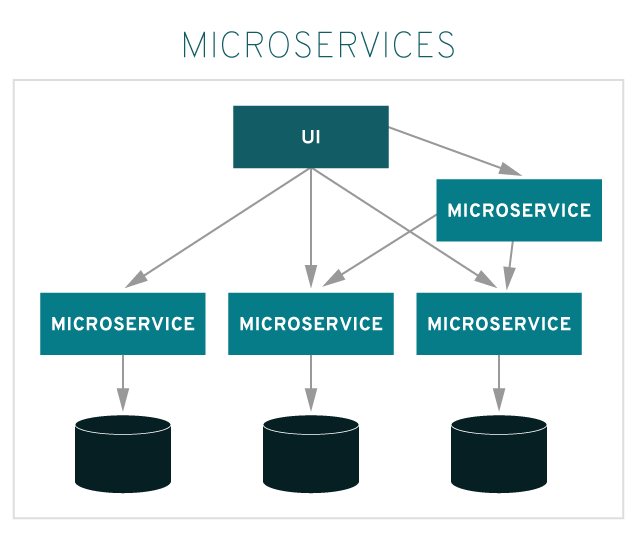
\includegraphics[width=0.7\linewidth]{imagenes/monolithic-vs-microservices}
		\caption{Estructura arquitectura microservicios}
		\label{fig:microservices}
	\end{figure}

	\section{Patrones de diseño}
	 En el momento de diseñar una arquitectura existen dos formas de actuar, diseñar una arquitectura desde cero o buscar soluciones ya propuestas a nuestro problema. Si elegimos la segunda opción existen patrones de diseño, patrones arquitectónicos y frameworks.
	 
	 Los patrones son una forma reutilizable de resolver problemas comunes. Los primeros definidos en arquitectura civil se encuentran en el libro “A pattern language” \cite{PatternLanguage}, en él se describen los patrones con un nombre, de tal manera que con hacer referencia a este, cualquier arquitecto será capaz de entender que solución se está usando sin tener que entrar en detalles. Sin embargo en la arquitectura de software no aparecieron hasta 1994 en un libro que a día de hoy sigue siendo un modelo de referencia\cite{gamma2002patrones}.
	 
	 Los patrones definidos en el libro \cite{gamma2002patrones} se dividen en función del problema a resolver:
	 
	 \begin{itemize}
	 	\item Patrones creacionales: éstos son los utilizados para facilitar la creación de nuevos objetos. Los más conocidos son:	 	
	 	\begin{itemize}
	 		\item Abstract Factory: Contiene una interfaz que otorga la creación de objetos relacionados, sin tener que especificar cuáles son las implementaciones concretas.
	 		\item Factory Method: Contiene un método de creación que delega en las subclases la implementación de dicho método.
	 		\item Builder: Con un mismo proceso de construcción nos sirve para crear diferentes representaciones, separando la creación de un objeto complejo de su estructura.
	 		\item Singleton: Solo se permite la creación de una instancia de una clase en nuestro programa y se proporciona un acceso global a él.
	 		\item Prototype: Un objeto se crea a partir de la clonación de otro objeto, es decir, se crea basándose en unas plantillas.
	 	\end{itemize}
 	\item Patrones estructurales: éstos nos facilitan la modelización de nuestro software, definiendo la forma en que las clases se relacionan entre sí. Los más conocidos son:
 	\begin{itemize}
 		\item Adapter: Mediante un objeto intermedio, se pueden comunicar dos clases con distinta interfaz. 
 		\item Bridge: Se crea un puente entre la abstracción y la implementación, para que puedan evolucionar independientemente.
 		\item Composite: Sirve para crear objetos contenidos en un árbol donde todos los elementos emplean una misma interfaz.
 		\item Decorator: Se añade funcionalidad extra a un objeto (de forma dinámica o estática) sin cambiar su comportamiento.
 		\item Facade: Objeto que crea una interfaz para poder trabajar con otra parte más compleja. Un ejemplo podría ser: crear una fachada para trabajar con una librería externa.
 		\item Flyweight: Para ahorrar memoria, gran cantidad de objetos comparten un objeto con las mismas propiedades.
 		\item Proxy: Clase que funciona como interfaz destinada a cualquier otra cosa: conexión a Internet, archivo en disco, etc.
 	\end{itemize}
 	\item Patrones de comportamiento: Se usan para gestionar algoritmos, relaciones y responsabilidades entre objetos. Los más conocidos son: 
 	\begin{itemize}
 		\item Command: Objetos que necesitan para ejecutarse, contener una acción y sus parámetros. 
 		\item Chain of responsibility: Permite pasar solicitudes a lo largo de una cadena de receptores. Al recibir una solicitud, cada controlador decide procesar la solicitud o pasarla al siguiente de la cadena.
 		\item Interpreter: Define una representación y el mecanismo para poder evaluar una gramática. El árbol de sintaxis del lenguaje se modela mediante el patrón Composite.
 		\item Iterator: Nos permite movernos por los elementos de forma secuencial sin necesidad de conocer su implementación.
 		\item Mediator: Objeto que contiene un conjunto de objetos que interactúan y se comunican entre sí.
 		\item Memento: Permite restaurar un objeto a un estado anterior.
 		\item Observer: Objetos que pueden unirse a una serie de eventos que otro objeto va a producir para estar informados cuando esto cambie.
 		\item State: Modifica el comportamiento de un objeto en el tiempo de ejecución.
 		\item Strategy: Selecciona el algoritmo que ejecuta ciertas acciones en tiempo de ejecución.
 		\item Template Method: Nos permite conocer la forma del algoritmo.
 		\item Visitor: Separa el algoritmo de la estructura de datos que se utilizará a la hora de ejecutarlo, por lo que se pueden añadir nuevas opciones sin tener que ser modificadas.
 	\end{itemize}
	 \end{itemize}
 \section{Patrones de arquitectura}
 Por otra parte también existen los patrones arquitectónicos o arquetipos, los cuales tienen un nivel superior de abstracción, es decir, no especifican cómo escribir el código, pero sí cómo debe estar organizado y que elementos son importantes en la aplicación. Estos al igual que los patrones de diseño, solucionan problemas recurrentes de una forma reutilizable.
 
 Los patrones de arquitectura más usados son:
 	\begin{itemize}
 	\item Programación por capas: Utilizada para estructurar programas que pueden descomponerse en subtareas. Normalmente cuenta con tres capas, en una de ellas se implementa la lógica de negocio, en otra los datos y en otra la presentación de los datos ya tratados. Es uno de los arquetipos mas usados a día de hoy.
 	\item Cliente-servidor: Este patrón consta de dos partes: un servidor y múltiples clientes, el servidor será el que de servicio a diversos componentes del cliente y los clientes solicitarán servicio al servidor. En esta arquitectura se separan las capas en varias maquinas físicas, normalmente se utiliza 2 o 3 niveles. Si utilizáramos dos niveles tendríamos la capa de presentación en una maquina del cliente y el tratado de los datos con la base de datos en otra máquina. En la de 3 niveles se pondría cada capa en un servidor diferente con la mejora de escalabilidad.
 	\item Arquitectura orientada a servicios: Es la que da soporte a los requerimentos del negocio mediante la creación de servicios. Un servicio corresponde a un requerimento funcional del negocio, por ejemplo: 
 	Un cliente necesita saber el stock de un determinado producto, por lo que se crea un servicio que consulte en la base de datos la cantidad de producto disponible.
 	\item Arquitectura de microservicios: Utilizada para crear aplicaciones usando un conjunto de pequeños servicios, los cuales se comunican entre sí pero se ejecutan de forma individual.
 	\item Pipeline: Utilizado para organizar sistemas que procesan una sucesión de datos. Estos datos pasan a través de tuberías (que son combinación de comandos que se ejecutan de forma simultanea, donde el resultado de la primera se envía de entrada para el siguiente). Las tuberías se usan para almacenar datos en buffer o para la sincronización de estos.
 	\item Arquitectura en pizarra: Se utiliza para la resolución de problemas de los cuales se desconoce su estrategia. Está formado por tres componentes:
 	\begin{itemize}
 		\item \textbf{Pizarra:} memoria que contiene todos los objetos. 
 		\item \textbf{Fuente de conocimiento:} son módulos especializados. 
 		\item \textbf{Componente de control:} encargado de seleccionar y ejecutar los módulos.
 	\end{itemize}
 	\item Arquitectura dirigida por eventos: Maneja principalmente los eventos y está formado por cuatro componentes que son: fuente de evento, escucha de evento , canal y bus de evento.
 	\item Peer-to-peer: Se llama pares a las componentes individuales y estos pueden funcionar como servidor, dando servicio a otros pares, o como cliente, pidiendo servicio a otros pares.
 	\item Modelo Vista Controlador: Divide un programa interactivo en tres partes:
 		\begin{itemize}
 			\item \textbf{Modelo:} está formado por los datos básicos y contiene la funcionalidad del programa. 
 			\item \textbf{Vista:} maneja la visualización de la información. 
 			\item \textbf{Controlador:} encargado de controlar la entrada (teclado y ratón) del usuario e informar al modelo y la vista de los cambios de acuerdo a los requerimentos.
 		\end{itemize}
 	Permite desacoplar los componentes y reutilizar código más eficiente. 
 \end{itemize}

\section{Frameworks}
 Otra opción para no tener que diseñar una arquitectura desde cero sería la utilización de frameworks. Estos son estructuras de software ya implementadas en las que un programador puede apoyarse para desarrollar un proyecto propio. Los frameworks están implementados y siguen tanto los patrones de software como los patrones de arquitectura y suelen incluir ficheros de configuración, librerías, etc.
 
 Existen frameworks para prácticamente todos los lenguajes de programación, con ellos solo se implementarían los requisitos funcionales del producto, eso sí, es importante valorar y elegir el framework que mejor se adapta al problema que vas a resolver.
 
  \begin{figure}
 	\centering
 	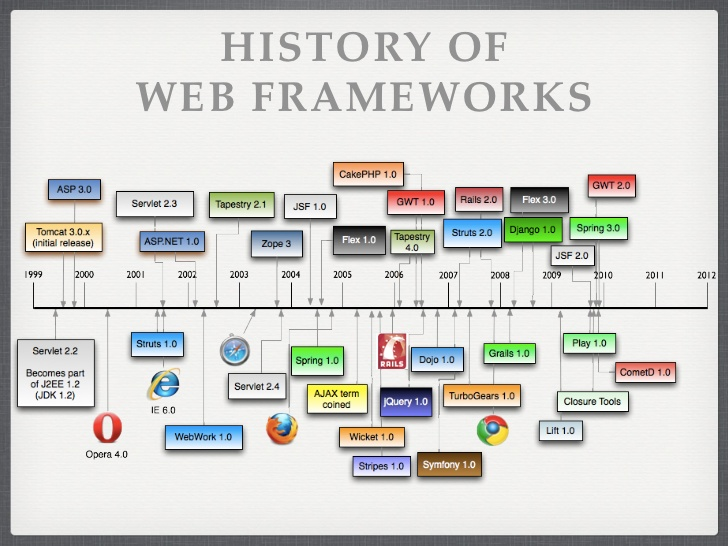
\includegraphics[width=0.7\linewidth]{imagenes/the-future-of-web-frameworks-11-728}
 	\caption{Historia de los Web Frameworks}
 	\label{fig:webFrameworks}
 \end{figure}

 Los frameworks de Java más utilizados en los últimos tiempos son Spring y Struts.
 
 Spring surgió en 2003 de la mano de Rod Johnson, la idea de este framework es agilizar y estandarizar la creación de proyectos de una misma arquitectura. 
 
 Struts nació en 2001 y está basado en la arquitectura Modelo Vista Controlador, el cual, permite gracias a las anotaciones poder configurar este modelo. Posteriormente, en 2004, surgió Stripes con la misma arquitectura pero con la finalidad de ser más ligero y eficiente.
 
 Existen framework de otros lenguajes de programación como por ejemplo Angular lanzado en septiembre de 2016. Está implementado en Typescript y orientado al desarrollo del Front-end de aplicaciones web. Este framework es propiedad de Google aunque es de código libre.
 
 React es otro framework para el desarrollo de Front-end. Contiene una serie de librerias de Javascript para construir las aplicaciones web mas fácilmente. Éste es propiedad de Facebook.
 
 Ionic surgió en 2013, siempre ha ido de la mano con Angular, desde AngularJs hasta las últimas versiones del mismo. Ionic está diseñado para desarrollar aplicaciones híbridas, según este artículo de next-u \cite{AppHibridas} “Las aplicaciones híbridas son aplicaciones móviles diseñadas en un lenguaje de programación web (HTML5, CSS o JavaScript), junto con un framework (Cordova) que permite adaptar la vista web a cualquier vista de un dispositivo móvil. Es decir, no son más que una aplicación construida para ser utilizada o implementada en distintos sistemas operativos móviles evitándonos la tarea de crear una aplicación para cada sistema operativo.”
 
 \subsection{Frameworks de Java para microservicios}
 Por otra parte existen bastantes frameworks que se basan en Java y ofrecen una arquitectura de microservicios, éstos han surgido de las grandes empresas del sector como Oracle, Spring, Eclipse. Entre ellos encontramos:

 \begin{itemize}
 	\item Spring Boot: Es una capa de personalización sobre el famoso framework Spring, que ofrece un arquetipo de un microservicio básico, ampliable fácilmente con poco desarrollo. Por ejemplo Gustavo Peiretti en el articulo \cite{StrategySpringBoot}, propone una implementación de un patrón strategy desarrollado con Spring Boot.
 	\item Cricket: Es un framework para implementación de arquitectura dirigida por eventos. Contiene un servidor HTTP incorporado, serialización de Java a JSON automática, gestión de usuarios y accesos, bases de datos integradas como H2 y un planificador de eventos. Con todo ello se puede construir una aplicación fácilmente.
 	\item Dropwizard: Es un framework para arquitectura de microservicios por capas, para utilizar este solo es necesario importarlo en la aplicación y usar todas las librerias que este incluye.
 	\item Eclipse MicroProfile: En junio de 2018 consiguió cubrir todas las necesidades de la arquitectura. Cuenta al igual que Spring con una web donde obtener un arquetipo de la aplicación con las dependencias que se necesiten.
 	\item Helidon: Es de las últimas incorporaciones en la arquitectura. Pertenece a la compañía Oracle que lo utilizó internamente bajo el nombre “Java for Cloud” y que finalmente se ha liberado para todo el público. 
 \end{itemize}
	
	\section{Bases de datos}
	En el proceso de diseño de una arquitectura otro módulo fundamental es el almacenamiento de los datos que vamos a utilizar, para ello usamos las bases de datos.

	Estas se pueden definir como un conjunto de información relacionada que se encuentra agrupada o estructurada.
	
	El concepto de bases de datos ha estado siempre ligado a la informática, éstas son sistemas formados por grupos de datos almacenados en discos, que permiten la consulta, modificación y borrado de los mismos. Se crearon para poder almacenar grandes cantidades de información. 
	
	En la década de los 70, Edgar Frank Codd, científico informático inglés conocido por sus participación en la teoría de bases de datos relacionales, definió el modelo relacional  a través de su artículo “Un modelo relacional de datos para grandes bancos de datos compartidos”\cite{RelationalModel}.
	
	Larry Ellison, basándose en el trabajo de Edgar F. Codd, creó el “Relational Software System” más conocido como Oracle Corporation, el sistema de gestión de bases de datos relacional más conocido actualmente.
	
	En la década de los 80 se desarrolló SQL un lenguaje de acceso a bases de datos relacionales que permite realizar consultas y cambios de forma sencilla. En los 90 se actualizó SQL y se agregaron: expresiones regulares, consultas recursivas, disparadores y algunas características orientadas a objetos.
	
	En la actualidad, las tres grandes compañías que dominan el mercado de las bases de datos son IBM, Microsoft y Oracle. En el campo de internet, la compañía que más información genera es Google.
	
	No fue hasta la década de los 2000 cuando surgieron las bases de datos NoSQL que son las que no contienen un identificador para relacionar un conjunto de datos con otro. La información se organiza en documentos y es útil cuando no tenemos claro lo que se va a almacenar.
	
	La más exitosa en bases de datos no relacionales es MongoDB seguida por Redis, Elasticsearch y Cassandra.
	
	\subsection{Pros y contras bases de datos relacionales}
	Ventajas:
	 \begin{itemize}
		\item Existe gran variedad de información para poder realizar cualquier tipo de desarrollo o consulta, gracias a sus años de madurez.
		\item Asegura que la información no se va a completar si a mitad de una operación realizada en base de datos ocurre un problema.
		\item Tiene los estándares bien definidos.
		\item Es sencillo a la hora de programar operaciones.
	\end{itemize}
	Inconvenientes:
		 \begin{itemize}
		\item Estas bases de datos tienden a crecer demasiado, por lo que aumenta el tiempo de respuesta.
		\item Se tendrá que reestructurar la base de datos de una empresa debido a que ésta realice algún cambio en sus sistemas informáticos.
		\item No garantizan el buen funcionamiento si el sistema operativo donde se va a instalar no cumple con los requerimientos mínimos.
	\end{itemize}

	\subsection{Pros y contras bases de datos no relacionales}
		Ventajas:
	\begin{itemize}
		\item Adaptabilidad para crecimientos o cambios a la hora de almacenar la información, si se necesita un nuevo campo en la base, se agrega sobre el documento y el sistema sigue operando sin tener que añadir nuevas configuraciones.
		\item Crecimiento horizontal. Si la actuación de los servidores disminuye durante la operación, existe la posibilidad de instalar nuevos nodos que distribuyen la carga de trabajo, de ahí, crecimiento horizontal.
		\item No es necesario contar con servidores con gran cantidad de recursos disponibles para realizar operaciones, si no que pueden empezar con un número de recursos limitado y dependiendo de las necesidades ir creciendo sin tener que detener las operaciones.
		\item Cuenta con un algoritmo interno que reformula las consultas de los usuarios o de las aplicaciones programadas para no sobrecargar a los servidores.
	\end{itemize}
	Inconvenientes:
	\begin{itemize}
		\item Como no nos garantiza que si la operación falla se complete la información, esta en ocasiones es inconsistente.
		\item Dado que es un modelo bastante nuevo, se necesitan conocimientos elevados en el uso de esta herramienta, ya que las operaciones son limitadas.
		\item No tiene un estándar de lenguaje definido.
		\item No contiene una interfaz gráfica por lo que es necesario hacer todo mediante consola.
	\end{itemize}

\section{Microservicios}

Una arquitectura de microservicios es útil para desarrollar una aplicación software dividiéndola en una serie de pequeños servicios, los cuales se ejecutan de forma independiente y se comunican entre sí, por ejemplo, a través de peticiones HTTP a sus API.

Tiene que haber un número mínimo de servicios encargados de gestionar los procesos en común. Cada microservicio es pequeño y se corresponde con un área de la aplicación. Cada uno es independiente, pudiéndose programar en lenguajes diferentes y su código debe poder ser implementado sin que afecte a los demás.

Cada microservicio no tiene definido ni el tamaño, ni cómo se tiene dividir la aplicación pero en el libro “Building Microservices”, \cite{BuildingMicroservices}se caracteriza un microservicio como “algo que a nivel de código podría ser reescrito en dos semanas”.

\subsection{Pros y contras de los microservicios}
Ventajas:
\begin{itemize}
	\item Concede a los desarrolladores la libertad de implementar y desplegar los servicios de forma independiente.
	\item Los microservicios se pueden desarrollar con un equipo de trabajo mínimo.
	\item Para cada módulo, existe la posibilidad de utilizar lenguajes diferentes.
	\item Con el uso de contenedores el desarrollo y despliegue de la App es mucho más rápido.
	\item Son fácilmente escalables.
\end{itemize}
Inconvenientes:
\begin{itemize}
	\item Las pruebas pueden resultar complicados debido al despliegue distribuido.
	\item Con un gran número de servicios se puede dar lugar a grandes bloques de información para gestionar.
	\item Si contamos con un gran número de servicios, a la hora de integrarlos y gestionarlos puede resultar muy complicado.
	\item Esta tecnología suele incurrir en un alto consumo de memoria.
	\item Fragmentar una aplicación en diferentes microservicios puede llevar muchas horas de planificación.
\end{itemize}

\subsection{Ejemplos de empresas que utilizan microservicios}

Para poder contemplar hasta dónde ha llegado la arquitectura de microservicios observamos algunas grandes marcas que lo han implementado. Webs de aplicaciones a gran escala han decidido utilizar los microservicios en vistas de productos mucho más simples, efectivos y rápidos. Encontramos estas compañías:
\begin{itemize}
	\item \textbf{Netflix:} Esta plataforma tiene una arquitectura generalizada que desde hace un par de años se pasó a los microservicios. A diario recibe una media de mil millones de llamadas a sus diferentes servicios y es capaz de adaptarse a más de 800 tipos de dispositivos mediante su API de streaming de vídeo.
	\item \textbf{Amazon:} No tiene soporte para tantos dispositivos como Netflix, pero tampoco es algo fundamental en su sector. Se cambió hace tres años a la arquitectura de microservicios siendo una de las primeras compañías que la implementan en producción. No hay cifra aproximada de la cantidad de solicitudes que pueden recibir a diario, pero no son pocas. 
	\item \textbf{Ebay:} Es una de las empresas con mayor visión de futuro, siendo pionera en la adopción de tecnologías como Docker. Su aplicación principal comprende varios servicios autónomos, y cada uno ejecutará la lógica propia de cada área.
\end{itemize}




\section{Comparación de SOA con Microservicios}
Primero surgió la arquitectura orientada objetos y más adelante la orienta a componentes. Pero no fue hasta 1996 cuando se desarrolló por primera vez SOA. Con ésta se desarrollaban todos los servicios necesarios y se empaquetaban en un archivo WAR para poder desplegarse en un servidor de aplicaciones, como por ejemplo Tomcat, que se encontraba dentro de una máquina. Esto puede verse en la figura \ref{fig:soavsmicroservicios}.

\begin{figure}
	\centering
	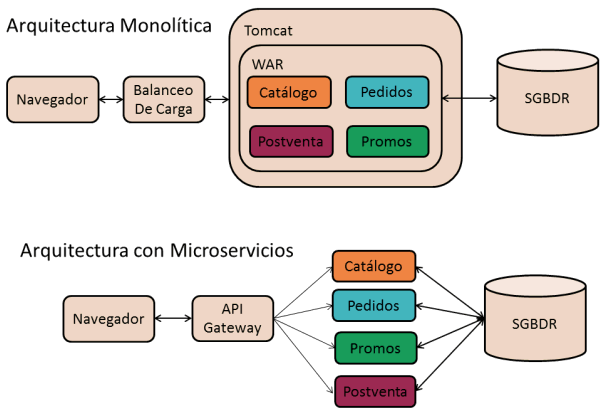
\includegraphics[width=0.7\linewidth]{imagenes/soavsmicroservicios}
	\caption{Arquitectura monolítica frente microservicios}
	\label{fig:soavsmicroservicios}
\end{figure}

Todos estos servicios tenían que estar implementados en el mismo lenguaje y no se les podía asignar más recursos a cada uno de ellos. Era asignado a todo el conjunto, dividiendo el archivo WAR en varias máquinas o réplicas de la misma. Para ello se necesitaba un balanceador de carga que determinaba que máquina iba a atender la petición.

Todo esto era suficiente para las empresas. A día de hoy cuando una aplicación monolítica (SOA) crece demasiado es difícil mantenerla y añadir nuevas funcionalidades, ya que cada línea modificada implica re-desplegar toda la aplicación, lo que puede llevar mucho tiempo pues en los despliegues están involucrados varios departamentos de la empresa que impide al equipo seguir desarrollando. También es complicado encontrar el origen de algún error en el código.

La necesidad por resolver todos estos problemas desembocó en la arquitectura de microservicios. La primera vez que se mencionó la palabra "microservicios" fue en 2011 en una conferencia sobre computación en la nube, donde el Dr. Peter Rogers\cite{breveHistoria} se refirió a ello para describir la arquitectura que estaban usando grandes empresas como Netflix, Facebook, Amazon o PayPal. 

Los microservicios gestionan la complejidad dividiendose funcionalmente en un conjunto de servicios pequeños e independientes. Con esto se consigue que el equipo de desarrollo sea capaz de implementar varias funcionalidades a la vez, sin tocar el código de otra funcionalidad y desplegar cada módulo por separado tal y como se ve en la figura \ref{fig:soavsmicroservicios} donde cada microservicio está separado del resto y pueden o no tener una base de datos común.

El cambio más notable respeto a SOA es que los equipos de desarrollo tienen una mayor responsabilidad, lo que se traduce en una gran facilidad, ya que manejan todo lo siguiente:  proceso de desarrollo, despliegues en distintos entornos, gestión de contenedores como Kubernetes, etc. Todo esto antes se tenía que realizar en otros departamentos de la empresa aumentando tiempos de producción. La arquitectura de microservicios resuelve todos los problemas que presenta SOA y cada vez es más popular, pero aún está en su base de inicio como se menciona en el articulo\cite{Dragoni2017} y aún le queda mucho por mejorar y evolucionar. 

Rajest RV en su libro "Spring Microservices"\cite{rv2016spring} nos muestra el gráfico \ref{fig:desarrollomonovsmicro} en el que se observa como es más rápido y ágil el desarrollo de aplicaciones con microservicios frente a aplicaciones tradicionales. Menciona que, "Los microservicios prometen más agilidad, velocidad de entrega y escala. En comparación con las aplicaciones monolíticas tradicionales." 

\begin{figure}
	\centering
	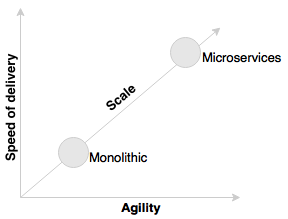
\includegraphics[width=0.7\linewidth]{imagenes/desarrolloMonovsMicro}
	\caption{Eficiencia microservicios frente SOA}
	\label{fig:desarrollomonovsmicro}
\end{figure}

Un aspecto a mejorar es la seguridad, ya que cuando se descompone una aplicación en cientos de microservicios aparecen dificultades en la depuración, monitoreo, auditoría y análisis de toda la aplicación. Los atacantes podrían aprovechar esta complejidad para atacar. 

Lo que sí es seguro es que han surgido para quedarse y cada vez más empresas están empezando a utilizar los microservicios.

\subsection{Ejemplo de visión monolítica vs visión de microservicio}

Accedemos a una página web de una tienda para realizar compras.

Hay un servidor que está ejecutando el código de la aplicación y de vez en cuando se conecta a una base de datos para recuperar información.
Cuando un usuario compra un producto vía web, se mostrarán los productos disponibles. La aplicación responderá según haya sido programada y mostrará el inventario, pagos o envíos. Esta información se empaqueta en un único archivo ejecutable. De ahí el nombrarlo como arquitectura monolítica.

Si se realiza un cambio en cualquiera de los módulos, se tendrá que subir a producción un código nuevo aunque los otros módulos no hayan sido modificados. Si la aplicación no es compleja, la subida será sencilla ya que en este caso tenemos un solo archivo ejecutable.

En el caso de microservicios, en vez de tener un único ejecutable, cada componente del sistema es un único servicio que se comunicará con los otros a través de llamadas.

Contamos con una interfaz web en la que interactúan los usuarios y por debajo los servicios de pagos, inventario y envíos.

Con respecto a la visión monolítica tenemos:

\begin{itemize}
	\item Los microservicio pueden desplegarse de manera independiente: si realizamos un cambio en uno de los módulos, no se verán afectados los otros módulos y solo tendremos que subir ese módulo.
	\item Es fácil de entender y dividir, pues las secciones del negocio están bien separadas.
	\item Cada microservicio es multifuncional: tiene una parte de base de datos, de Back-end y es independiente de los demás.
\end{itemize}

\begin{figure}
	\centering
	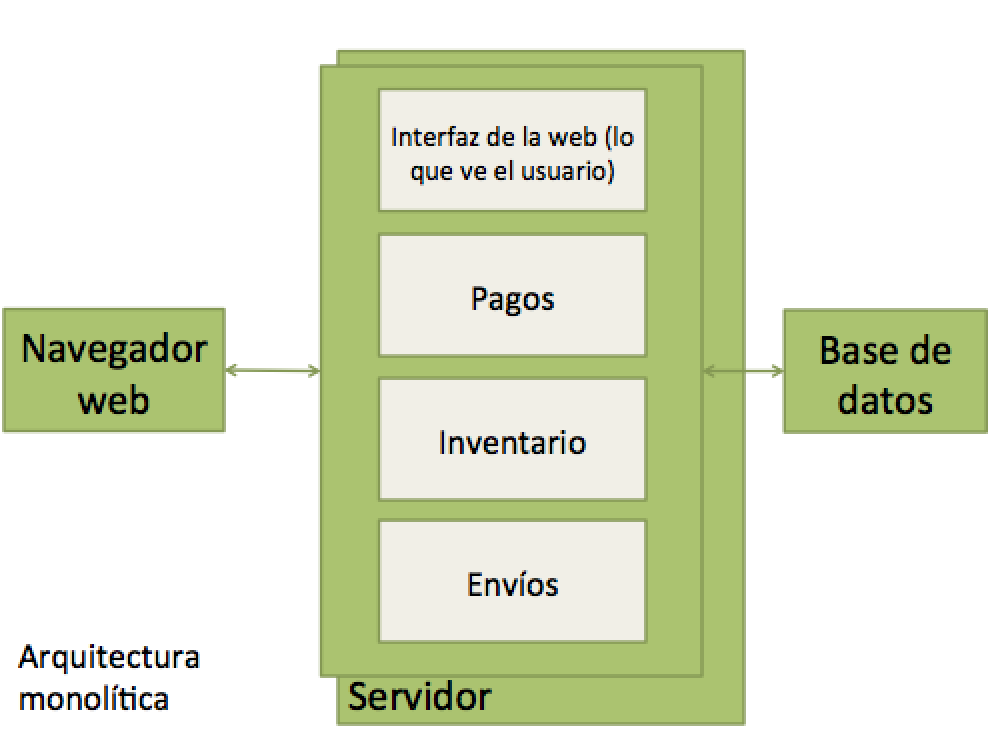
\includegraphics[width=0.7\linewidth]{imagenes/monolithic}
	\caption{Ejemplo de arquitectura monolitica(SOA)}
	\label{fig:monolithic}
\end{figure}
\begin{figure}
	\centering
	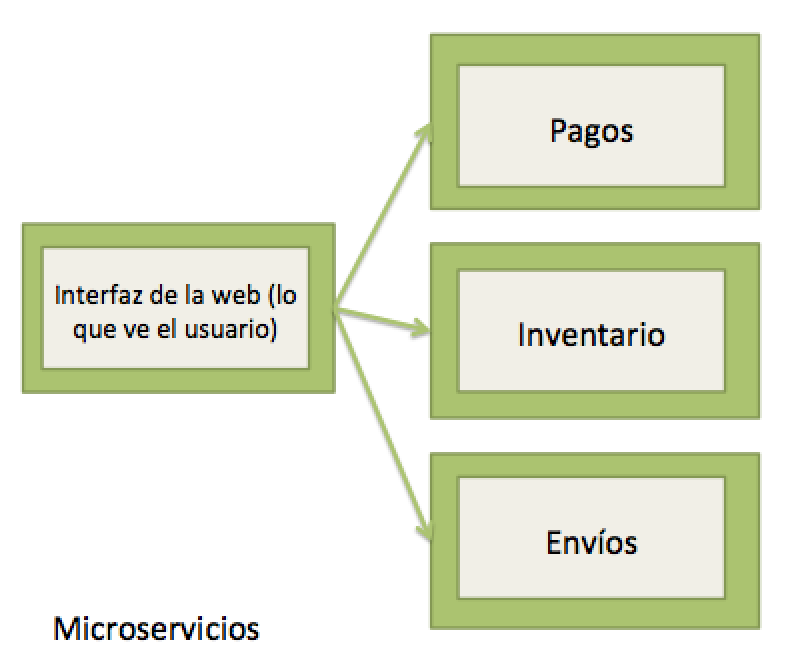
\includegraphics[width=0.7\linewidth]{imagenes/microservices}
	\caption{Ejemplo arquitectura microservicios}
	\label{fig:microservicesGrafic}
\end{figure}


\chapter{Justificación de la solución propuesta}

Analizando los requisitos que tenemos nos quedaríamos con 3 tipos de arquitecturas candidatas, una sería la arquitectura en capas, otra la arquitectura orientada a servicios(SOA) y por ultimo la arquitectura de microservicios. 

Con cualquiera de ellas podríamos montar un servicio que hiciera lo que nosotros necesitamos, sin embargo, la única que ofrece escalabilidad y alta disponibilidad es la arquitectura de microservicios. Además se adapta perfectamente a la filosofía de la arquitectura, ya que cada servicio tiene que ser pequeño. Al estar en la nube no necesitamos servidores físicos, se contratará en cada momento lo que se necesite y así se reducen gastos.

Para el desarrollo de la aplicación hemos elegido Spring Boot como framework de microservicios. Éste cuenta con una web donde poder descargar un arquetipo, incluye todas las ventajas de Spring para el desarrollo en capas, que también vamos a necesitar y además es el más utilizado a día de hoy, por lo que es el que más soporte nos ofrece.

Para la gestión de dependencias elegimos Maven ya que es el más utilizado y totalmente dirigido para Java. Éste nos va a empaquetar la aplicación en un archivo jar compilandola y añadiendo las dependencias que necesite.

Vamos a utilizar Lombok para evitar código repetitivo en las clases, como getter, setter y constructores. Mediante anotaciones conseguimos todo esto en tiempo de ejecución. Ademas también nos ofrece una implementación del patrón de diseño builder.

La comunicación con el microservicio va a ser mediante REST que está basado en el protocolo HTTP que es simple y muy eficaz para realizar las distintas operaciones(verbos) en base de datos: añadir, recuperar, actualizar y eliminar, esto en REST seria PUT, GET, POST, y DELETE.

Todo servicio REST necesita un documento API donde se describa la entrada y salida de él, en este caso vamos a utilizar anotaciones de Swagger para que este documento se autogenere, además nos ofrece la posibilidad de llamar a traves de él, que es más visual que una llamada por Postman.

En la figura \ref{fig:capturaswagger} vemos los métodos a los que podemos llamar y dentro de los métodos tenemos la entrada salida y una descripción de que hace cada uno.
\begin{figure}
	\centering
	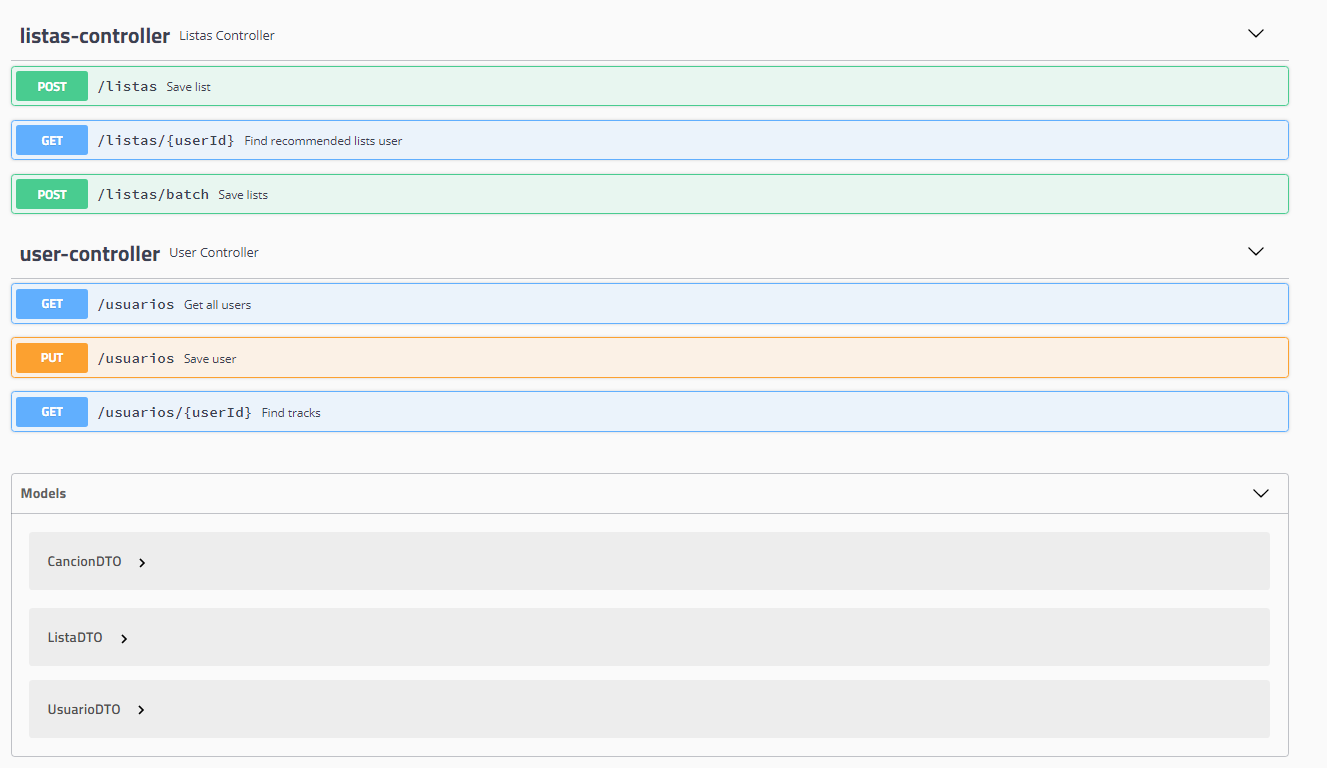
\includegraphics[width=0.7\linewidth]{imagenes/CapturaSwagger}
	\caption{API en Swagger}
	\label{fig:capturaswagger}
\end{figure}


Por otra parte para la base de datos, como tenemos los datos en formato JSON, lo ideal es una base de datos NoSQL para guardar directamente el JSON sin tener que hacer una conversión a tablas. Además es adaptable a cambios para que sea más mantenible y puede establecerse en la nube al igual que el microservicio para que la comunicación sea rápida. Al estar en la nube se adapta fácilmente a los requisitos de cada momento. Por ejemplo si en una campaña se necesita realizar muchas consultas a base de datos se puede ampliar los núcleos de esta para que responda más rápido.

Por tanto elegimos MongoDB como base de datos que al estar utilizando Azure se llama CosmosDB, la única diferencia es que se establece una capa de personalización para que sea más rápida y limitar el número de accesos en función a lo que se tenga contratado. También está preparada para trabajar con un número elevado de datos sin saturarse.

\chapter{Desarrollo de la aplicación}

El primer paso para desarrollar nuestra aplicación es tener un IDE instalado, en este caso usamos Eclipse.

\begin{figure}
	\centering
	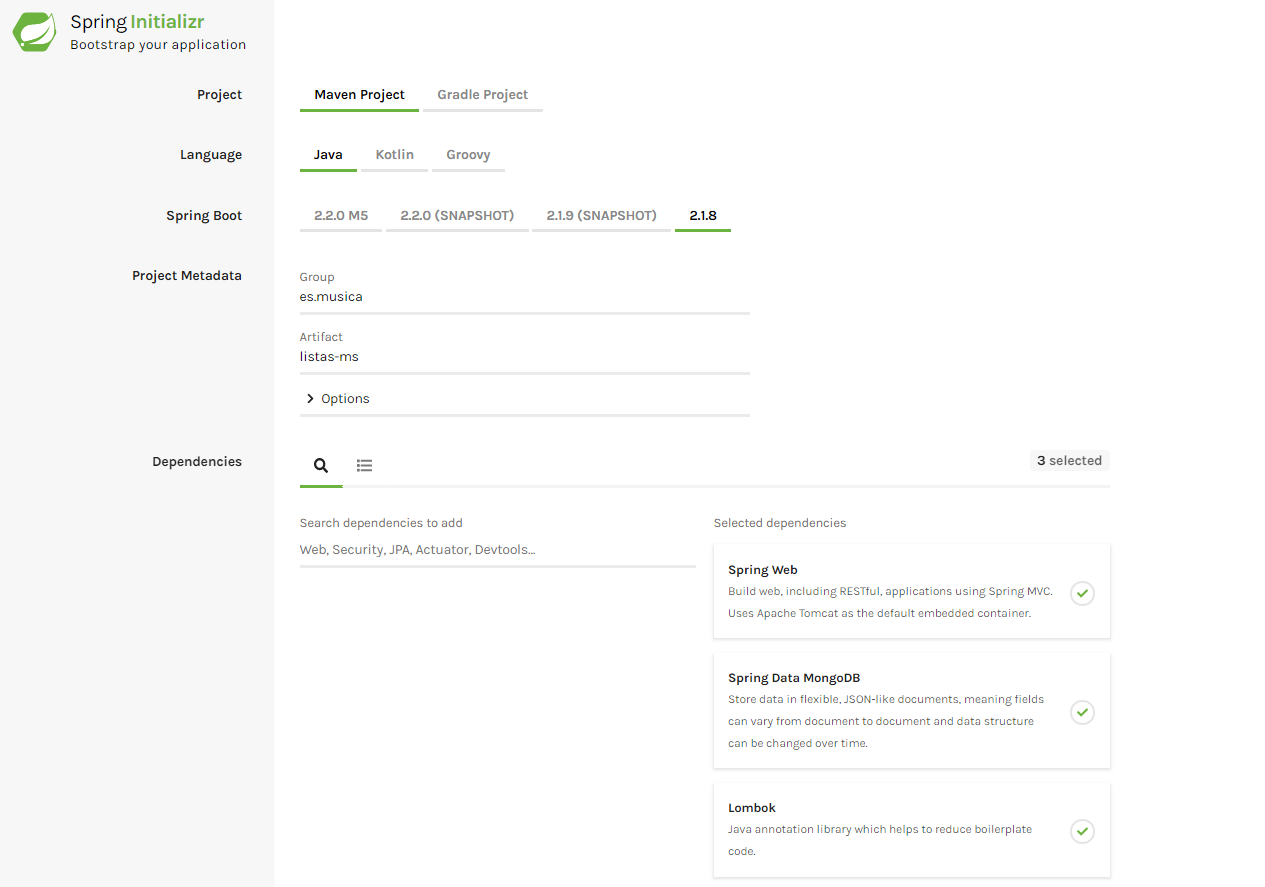
\includegraphics[width=0.7\linewidth]{imagenes/arquetipo}
	\caption{Ejemplo configuración arquetipo}
	\label{fig:arquetipo}
\end{figure}

Una vez que tenemos Eclipse instalado, nos dirigimos a la web https://start.spring.io/ para obtener un arquetipo de aplicación usando el framework Spring Boot. Como observamos en la figura \ref{fig:arquetipo} elegimos Maven para el control de dependencias, escogemos Java como lenguaje y por último las dependencias que queremos incluir, MongoDB, Spring Web, Lombok; nos faltarían las dependencias de Swagger pero esta web no las proporciona así que posteriormente las añadiremos.

Importamos en Eclipse el arquetipo descargado como proyecto Maven y al compilarlo se descargaran todas las dependencias incluidas en el fichero pom.xml, es el momento de añadir las dependencias de Swagger que vamos a necesitar.

\begin{figure}
	\centering
	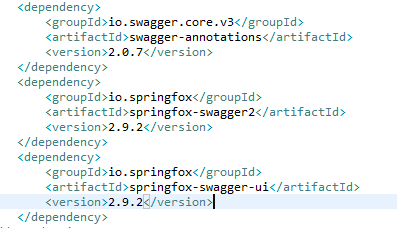
\includegraphics[width=0.7\linewidth]{imagenes/dependenciasSwagger}
	\caption{Dependencias Swagger necesarias}
	\label{fig:dependenciasswagger}
\end{figure}

Swagger es un software para diseñar, documentar y consumir servicios REST. En la figura \ref{fig:dependenciasswagger} podemos ver las dependencias necesarias para poder utilizarlo, la primera dependencia es para poder utilizar anotaciones de Swagger, y las dos siguientes son para que al desplegar la aplicación se incorpore un recurso donde visualizar el documento Swagger de nuestro código y así poder hacer llamadas a nuestros servicios, este documento lo vemos en la figura \ref{fig:capturaswagger}

Para configurar Swagger es necesario añadir la clase de configuración que se muestra en la figura \ref{fig:cofingswagger}. Con la anotación de la clase @EnableSwagger2 habilitamos la generación del dominio antes citado y además esta clase contiene un método donde configuramos de que paquete queremos que nos cree el API.

\begin{figure}
	\centering
	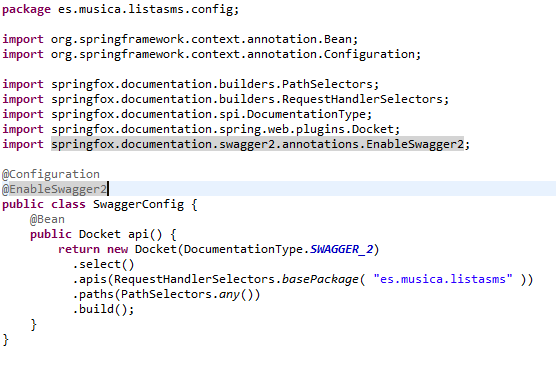
\includegraphics[width=0.7\linewidth]{imagenes/cofingSwagger}
	\caption{Clase configuración Swagger}
	\label{fig:cofingswagger}
\end{figure}


Creamos un repositorio en Github !!!!!!!!!!!!!!!!! para poder guardar lo que tenemos hasta ahora. Es recomendable ir subiendo al repositorio cada poco tiempo y agrupando una funcionalidad para poder volver a un commit concreto y resolver errores.

El arquetipo contiene una clase App la cual hay que ejecutar para levantar el microservicio en local, para hacerlo, al tener una dependencia de MongoDb tenemos que establecer la conexión con la base de datos.

Existen dos opciones: descargar MongoDB embebido y levantar una base de datos local o nuestro caso, crear en Azure una instancia de CosmosDB y configurar el microservicio para que apunte a esa base de datos. Para esta configuración creamos una clase de Java llamada MongoDbConfig y mediante la anotación @Value, obtenemos de application.properties la conexión a CosmosDB y el nombre de la base de datos. Una vez hecho esto ya podemos levantar el microservicio. Esta clase de configuración la podemos ver en la figura \ref{fig:configmongo}

\begin{figure}
	\centering
	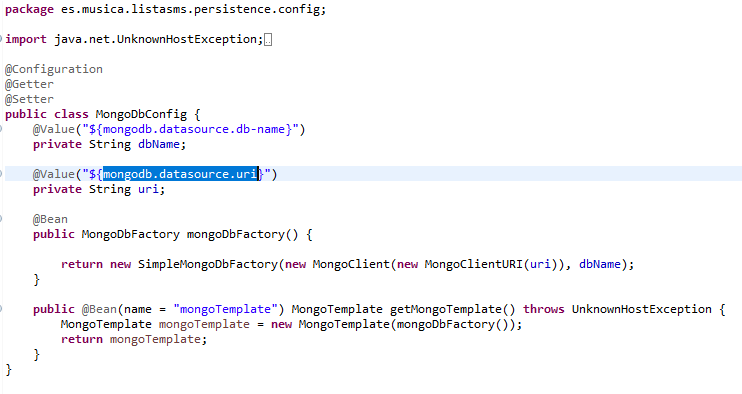
\includegraphics[width=0.7\linewidth]{imagenes/configMongo}
	\caption{Clase de configuración MongoDB}
	\label{fig:configmongo}
\end{figure}


\begin{figure}
	\centering
	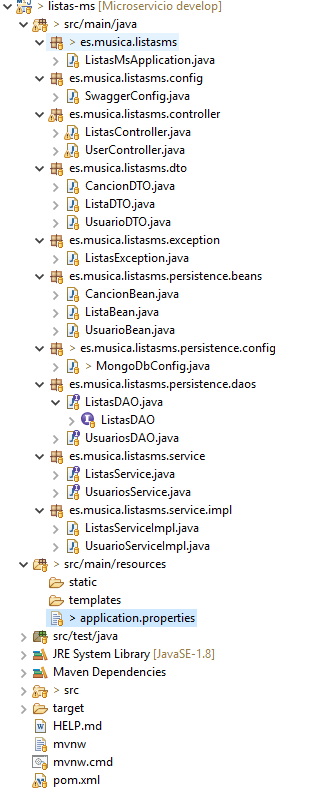
\includegraphics[width=0.7\linewidth]{imagenes/estructuramicroservicio}
	\caption{Estructura microservicio}
	\label{fig:estructura-microservicio}
\end{figure}

El siguiente paso consiste en crear las tres capas que vamos a utilizar; la capa de persistencia, donde se definen las querys, la capa de servicio donde se implementa la lógica de negocio y la capa de presentación donde se implementan los verbos HTTP con los que se va a llamar al servicio. En la figura \ref{fig:estructura-microservicio} se puede ver la estructura de capas que hemos utilizado.

Una buena práctica a la hora de programar en capas es, que los objetos de la capa de persistencia no deben exponerse a la capa de presentación. Por ello hemos creado unos objetos Bean que son: ListaBean, UsuarioBean y CancionBean, que sirven para mapear el contenido de la base de datos, es decir en la base de datos guardamos un JSON que se transforma en una lista de estos objetos.
Para las querys hemos utilizado el framework Spring Data, hemos creado una interfaz por colección en base de datos y dicha interfaz tiene que extender de MongoRepository, solo por ello tiene todos los métodos más usados como por ejemplo: dame todos los elementos, cuenta cuantos elementos hay, inserta un elemento, inserta muchos elementos, actualiza un elemento, etc. Además de ello si en la interfaz definimos un método teniendo en cuenta la sintaxis de Spring Data también funcionará. Por ejemplo en ListasDAO hemos creado el siguiente método:

List<ListaBean> findByTracksTrackUriIn(List<String> trackUris);

Si lo analizamos vemos que recibe una lista de String y devuelve una lista de ListaBean, Spring data transforma el nombre del método en una query. Con la palabra find indicamos que la operación que se va a realizar en base de datos es una búsqueda. ByTracks nos indica que la búsqueda se va a hacer en el objeto ListaBean  en el campo tracks, que es una lista de CancionBean; a continuación TrackUriIn va a buscar el atributo trackUri en los objetos CancionBean obtenidos y compara este campo con la lista que entra como parámetro. Por tanto lo que hace el método es buscar todas las listas de reproducción que contienen alguna de las canciones que se pasan como parámetro.

Una vez tenemos los métodos necesarios en la capa de persistencia, pasamos a la capa de servicio en la que vamos a crear una interfaz con los métodos que vamos a exponer en la capa de presentación. Nuevamente tenemos una interfaz para listas de reproducción y otra para usuarios. En las implementaciones de las interfaces es importante anotar las clases con @Service y los DAOs a los que vayamos a llamar con @Autowire para que se instancien.

En esta capa se llama a los métodos necesarios de la capa anterior y además puedes llamar a métodos de un servicio diferente, por ejemplo, si llamas al método de listas y le pasas un idUsuario tienes que llamar al servicio de usuarios para que te devuelva las canciones de éste y así poder filtrar en las listas por esas canciones, además tiene que hacer el mapeo entre los objetos beans y los objetos DTO que son los que se exponen en la salida.

La capa de presentación es la encargada de serializar un JSON a un objeto y en función del recurso, llamar a un servicio u otro. En ella se definen los recursos y los verbos de la petición. 

\chapter{Descripción API microservicio}

Hemos desarrollado una serie de servicios en cada controlador, estos pueden verse en las figuras \ref{fig:controllerlistas} y \ref{fig:controllerusuarios}. 

\begin{figure}
	\centering
	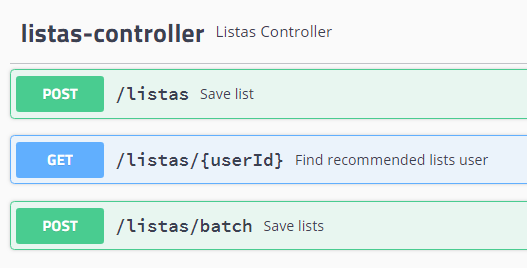
\includegraphics[width=0.7\linewidth]{imagenes/controllerListas}
	\caption{Recursos disponibles dentro del controller Listas}
	\label{fig:controllerlistas}
\end{figure}


\begin{figure}
	\centering
	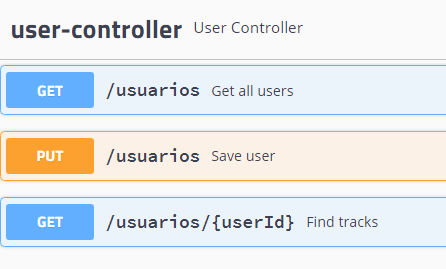
\includegraphics[width=0.7\linewidth]{imagenes/controllerUsuarios}
	\caption{Recursos disponibles dentro del controller Usuarios}
	\label{fig:controllerusuarios}
\end{figure}

En el controlador de listas hemos creado un recurso llamado /listas al que es posible acceder mediante el verbo POST y su función es almacenar en la base de datos una lista de reproducción nueva. El JSON de entrada necesario es el de la figura \ref{fig:jsonlista}.

\begin{figure}
	\centering
	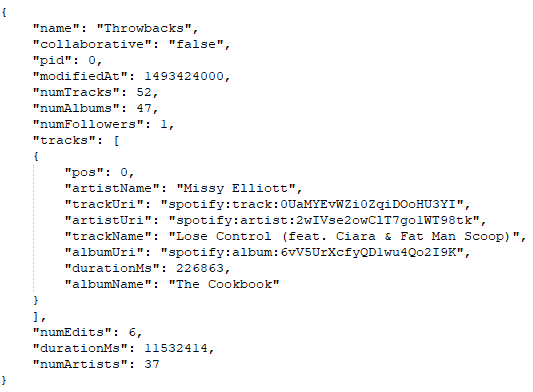
\includegraphics[width=0.7\linewidth]{imagenes/jsonLista}
	\caption{JSON ejemplo lista reproducción}
	\label{fig:jsonlista}
\end{figure}


Este JSON corresponde a una lista de reproducción con una única canción. Los campos que aparecen son los proporcionados por Spotify y simplemente se han renombrado para evitar el uso de caracteres como el guión bajo.

Al llamar al servicio con el JSON se creará un nuevo documento en la base de datos.

En el recurso /listas/\{userId\} mediante el verbo GET, al pasarle el id de usuario y un numero de canciones a coincidir, nos devuelve un listado en formato JSON con las listas de reproducción en las que el usuario tiene al menos el número, antes indicado, de canciones en común con la lista.

Por último en este controlador hemos añadido un recurso llamado /listas/batch y su función es la misma que la de /listas pero en la entrada recibe una lista de listas de reproducción y las da de alta en la base de datos.


En el controlador de usuarios hemos creado el recurso /usuarios al que es posible acceder mediante el verbo GET y nos devuelve un JSON con todos los usuarios dados de alta en base de datos.

Hemos creado otro recurso en /usuarios esta vez con el verbo PUT para crear un usuario con las canciones que ha escuchado en la base de datos. El JSON de entrada sería el de la figura \ref{fig:jsonusuario}.

\begin{figure}
	\centering
	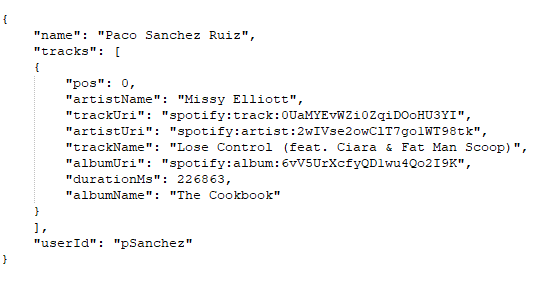
\includegraphics[width=0.7\linewidth]{imagenes/jsonUsuario}
	\caption{JSON ejemplo usuario}
	\label{fig:jsonusuario}
\end{figure}


Por último hemos creado un recurso llamado /usuarios/\{userId\} con el verbo GET que al pasarle el id de usuario nos devuelve ese usuario con las canciones que ha escuchado.

\chapter{Despliegue de la aplicación}

Para el despliegue de la aplicación en local lo primero es compilar el código mediante Maven. Para ello vamos a la ventana Run Configuration en Eclipse y creamos un nuevo Maven build como vemos en la figura \ref{fig:cleaninstallmaven}. En el campo base directory hay que poner lo que se muestra en la figura \ref{fig:cleaninstallmaven}. En el campo goals vamos a poner clean install para limpiar primero el proyecto y luego compilarlo. En el campo user settings se puede dejar así configurado por defecto si todas las dependencias son de internet o configurar un fichero personal donde se establezca a que repositorio ir a buscar las dependencias necesarias. En el campo Maven runtime se puede utilizar el Maven incluido en eclipse o una versión que nosotros descarguemos.

\begin{figure}
	\centering
	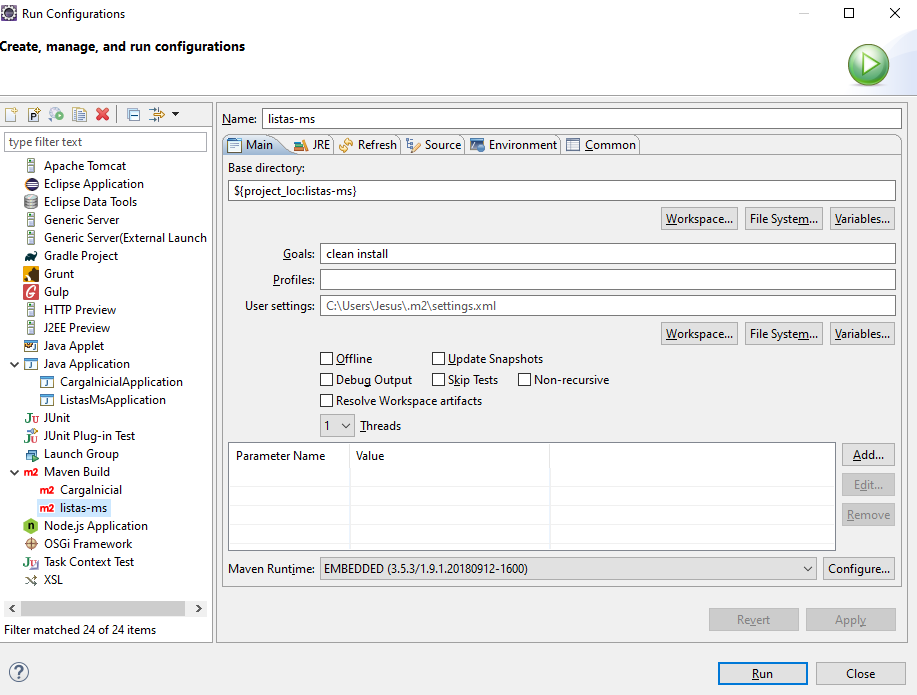
\includegraphics[width=0.7\linewidth]{imagenes/cleanInstallMAven}
	\caption{Configuración compilación mediante Maven}
	\label{fig:cleaninstallmaven}
\end{figure}

En la pestaña de JRE es importante seleccionar Java 8 o superior ya que utilizamos funcionalidades que no son compatibles con versiones anteriores y es necesario incluir la JDK y no la JRE como se ve en la figura \ref{fig:jremaven}.

\begin{figure}
	\centering
	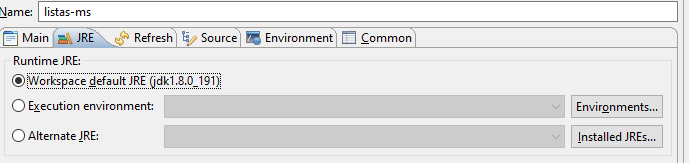
\includegraphics[width=0.7\linewidth]{imagenes/jreMaven}
	\caption{Configuración JRE proyecto}
	\label{fig:jremaven}
\end{figure}

Una vez se tiene todo esto seleccionado se procede a dar al botón de Run, la aplicación se compilará desde cero y se ejecutaran las clases de test existentes. Una vez concluido lo anterior, en la carpeta target, se habrá generado un archivo JAR.

Para desplegar la aplicación es necesario tener activa la base de datos a la que se va a conectar.

De nuevo iremos a la pantalla de Run Configuration, esta vez creamos una nueva configuración de Java Application como se muestra en la figura \ref{fig:configuraciondespliegue}. En el campo project se selecciona la raíz del proyecto y en el campo Main class, seleccionamos la ubicación de nuestra clase llamada ListasMsApplication.java, que es la que contiene el método main. Al dar al botón Run, se desplegará la aplicación. 

\begin{figure}
	\centering
	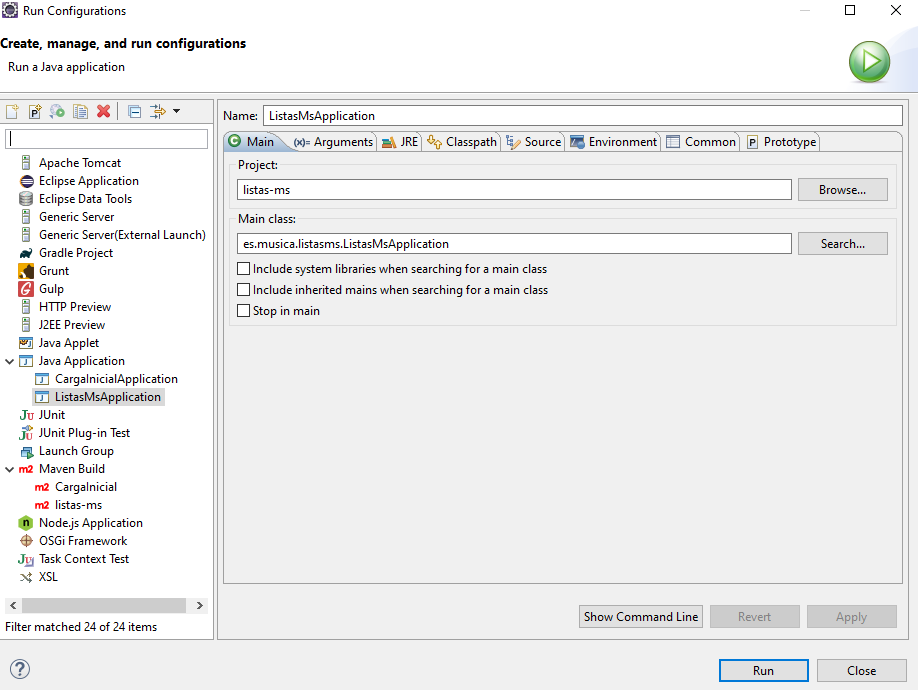
\includegraphics[width=0.7\linewidth]{imagenes/configuracionDespliegue}
	\caption{Configuración Run despliegue}
	\label{fig:configuraciondespliegue}
\end{figure}

Es posible acceder a la aplicación desde la siguiente dirección http://localhost:8080. Si queremos acceder a un recurso GET se puede hacer desde un navegador, si es otro tipo de recurso hay que hacerlo mediante Swagger o Postman. Todos los recursos están creados en las clases controller.

Además de los recursos creados por nosotros, se crean dos recursos de Swagger que son los llamados /swagger-ui.html\ref{fig:capturaswagger} y /v2/api-docs; el primero es la parte visual de Swagger y el segundo es el fichero .yml con el que se genera la parte visual de Swagger.

\chapter{Marco regulador}

No existen leyes que se apliquen en el desarrollo de un microservicio, ya que prácticamente todos los software que se utilizan son de código libre. Sin embargo si se ha de tratar con datos de clientes reales hay que tener en cuenta dos leyes:
\begin{itemize}
	\item Ley Orgánica de Protección de Datos Personales y garantía de los derechos digitales \cite{LeyProteccion}: En la ley Orgánica 3/2018, de 5 de diciembre, se establecen los principios de la protección de datos personales: exactitud, confidencialidad, consentimiento. Ya que vamos a almacenar datos de los usuarios, es necesario que cuando se cree un frontal que llame al servicio de insertar usuarios, antes se de consentimiento al uso de sus datos personales siempre bajo la ley.
	\item Ley General de Telecomunicaciones \cite{LeyComunicaciones}: En la ley 9/2014, de 9 de mayo, se estable en el articulo 43 que debemos cifrar toda la información que viaje mediante redes de comunicación. 
\end{itemize}

Por otra parte existen lo que se denomina buenas prácticas en el desarrollo que son consejos para que el código sea más limpio, legible, eficiente y mantenible. Estas buenas prácticas se pueden controlar a través de herramientas de calidad de código como por ejemplo Sonar.

\chapter{Entorno socio-económico}	

\section{Presupuesto}
En este punto vamos a calcular los costes del proyecto. Desde los costes de diseño, implementación y recursos hasta los servicios necesarios.

\subsection{Mano de obra}

El proyecto se ha desarrollado durante 8 meses con un total de 300 horas empleadas.

\begin{table}[H]
	\begin{center}
		\begin{tabular}{|c|c|c|}
			\hline
			Coste/Hora & Horas & Total \\
			(euros) &  & (euros) \\
			\hline \hline
			15 & 300 & 4500 \\ \hline
			
		\end{tabular}
		\caption{Coste personal.}		
		\label{costePersonal}
	\end{center}
\end{table}

Si este proyecto se desarrollara en una empresa, contaría con un arquitecto de sistemas que realice el diseño de la arquitectura y con un desarrollador para la implementación de la aplicación.

\subsection{Recursos físicos}
A continuación pasamos a evaluar los gastos relacionados con los recursos amortizables. 
Para estimar el precio de cada recurso, se ha calculado una media entre los diferentes precios de cada proveedor. 

La amortización corresponde a los meses de vida útil de cada recurso.
Para poder calcular el precio final hemos realizado las siguientes operaciones; el proyecto se ha desarrollado a lo largo de 8 meses por lo que hemos dividido el precio del recurso entre la amortización en meses y lo multiplicamos por la duración del proyecto.

Los recursos utilizados y sus costes son los siguientes:

\begin{table}[H]
	\begin{center}
		\begin{tabular}{|l|c|c|c|c|}
			\hline
			Recurso & Precio & Amortización & Coste mensual & Total \\
			 &  & (Meses) & (euros) & (euros) \\
			\hline \hline
			Ordenador portátil & 700 & 72 & 9,7 & 77,8 \\ 
			HP Pavilion DV6 &  &  &  &  \\ 
			\hline
			TeXstudio & 0 & 12 & 0 & 0 \\ \hline
			Eclipse & 0 & 12 & 0 & 0 \\ \hline
			NotePad ++ & 0 & 12 & 0 & 0 \\ \hline \hline
			Total & & & & 77,8 \\ \hline
			
		\end{tabular}
		\caption{Coste de recursos.}		
		\label{costeRecursos}
	\end{center}
\end{table}

\subsection{Servicios}
Hemos necesitado recurrir a una nube de desarrollo donde almacenar nuestra base de datos y para ello hemos utilizado Microsoft Azure. A continuación se muestra el presupuesto que nos ofrece este proveedor para tener una base de datos en la nube con alta disponibilidad. Cuando el servicio afronte menos número de peticiones se reducirá el coste. Al contratar estos servicios, el proveedor nos ofrece soporte gratuito.

\begin{table}[H]
	\begin{center}
		\begin{tabular}{|l|l|c|}
			\hline
			Tipo de servicio & Descripción & Coste estimado \\
			 &  & (euros) \\
			\hline \hline
			Azure CosmosDB & Escritura de una sola región - Europa Occidental; & 534,67 \\ 
			&  Pago por uso; 100 x 100 RU x 730 Horas; & \\
			& 50 GB de almacenamiento & \\ \hline \hline
			Total mensual &  & 534,67 \\ \hline
			
		\end{tabular}
		\caption{Costes Microsoft Azure.}
		\label{costeAzure}
	\end{center}
\end{table}

Para trabajos futuros sería necesario contratar AKS para poder gestionar los contenedores donde se desplegaría cada microservicio. Esto nos supondría un aumento de 87,6 Euros mensuales.

\subsection{Coste total}

Recopilando los presupuestos de mano de obra, recursos y servicios utilizados, el coste total de este proyecto sería el siguiente.

\begin{table}[H]
	\begin{center}
		\begin{tabular}{|l|c|}
			\hline
			Concepto & Total \\
			 & (euros) \\
			\hline \hline
			Mano de obra & 4500 \\ \hline
			Recursos & 77,8 \\ \hline
			Servicios & 1069,34 \\ \hline \hline
			Total & 5647,14 \\ \hline					
		\end{tabular}
		\caption{Costes Totales.}
		\label{costeTotal}
	\end{center}
\end{table}

\section{Impacto socio-económico}

Uno de los objetivos de desarrollar aplicaciones con microservicios es que éstas sean fácilmente mantenibles y que puedan evolucionar según las necesidades de la sociedad.

Una de las ventajas de implantar los microservicios en la nube es la mejor utilización de los recursos disponibles (energía, servidores) ya que permite aprovechar éstos al máximo de una manera eficiente y además se centraliza la ubicación de las maquinas en granjas de servidores que intentan abastecerse con tecnologías renovables.

Anteriormente, cuando esperabas un número grande de peticiones era necesario adquirir un gran número de servidores para poder dar servicio al pico de trabajo, esto suponía que una vez pasado el pico tenías una serie de recursos sin utilizar, esto lo solucionan los microservicios en la nube.

Por otra parte, un inconveniente de esto es, que para una aplicación pequeña que va a contar con mucho tráfico de datos, el coste es mucho mayor en la nube que teniendo un par de servidores.

\chapter{Conclusiones}

Hemos conseguido cumplir el objetivo de diseñar una arquitectura capaz de recibir multitud de peticiones.

Para la base de datos elegimos una en la nube, aunque ésta es la mejor opción, nos hemos dado cuenta que tiene un coste muy elevado para una pequeña aplicación ya que cobran por uso y almacenamiento. Sin embargo si que hemos podido ver que para el problema al que nos enfrentamos, la base de datos elegida es la ideal.

Implementar el microservicio ha sido una tarea de investigación ya que todas las tecnologías utilizadas son bastante novedosas y es complicado encontrar información al respecto. Pero gracias a ello hemos conseguido una aplicación limpia y fácilmente mantenible.

\section{Trabajos futuros}

A continuación explicamos los posibles trabajos futuros que podrían implementarse para mejorar o complementar nuestra aplicación.

\textbf{Aplicación Web}

Se podría desarrollar una aplicación web para visualizar los datos de formas más amigable.

\textbf{Nuevas funcionalidades}

Añadir nuevas funcionalidades sobre los datos existentes, como por ejemplo un recomendador de listas.

\textbf{Integración continua}

Se podría añadir la aplicación a un circuito de integración continua para su utilización en una empresa.
La aplicación pasaría por este circuito cada vez que se hiciera un cambio en una rama de Git:
\begin{itemize}
	\item Compilación con test del código.
	\item Validación de la calidad del código con una aplicación como por ejemplo Sonar.
\end{itemize}

Este tipo de circuitos se suelen realizar mediante la herramienta Jenkins

\textbf{Dockerización}

Por otra parte se podría dockerizar la aplicación para poder integrarla en un contenedor y desplegar éste en la nube.

\textbf{Gestión de contenedores}

Incluir un gestor de contenedores en Azure para gestionar el escalado y otras configuraciones de las aplicaciones que tengamos dockerizadas.





%----------
%	BIBLIOGRAFÍA
%----------	

%\nocite{*} % Si quieres que aparezcan en la bibliografía todos los documentos que la componen (también los que no estén citados en el texto) descomenta está lína

\clearpage
\addcontentsline{toc}{chapter}{Bibliografía}
\setquotestyle[english]{british} % Cambiamos el tipo de cita porque en el estilo IEEE se usan las comillas inglesas.
\printbibliography



%----------
%	ANEXOS
%----------	

% Si tu trabajo incluye anexos, puedes descomentar las siguientes líneas
%\chapter* {Anexo x}
%\pagenumbering{gobble} % Las páginas de los anexos no se numeran




\end{document}